% This template was originally by R. Jacob Vogelstein
% Updated on March 1, 2010 by Noah J. Cowan
% Updated in late 2016 by Jonathan Bohren ME'17

%%%%%%%%%%%%%%%%%%%%%%%%%%%%%%%%%%%%%%%%%%%%%%%%%
% Font size:        10pt, 11pt, 12pt
% Paper size:       letter
% Margin ordering:  oneside, twoside
% Draft mode:       draft (no figures), final
%%%%%%%%%%%%%%%%%%%%%%%%%%%%%%%%%%%%%%%%%%%%%%%%%
\documentclass[12pt,letterpaper,oneside,final]{thesis}

% use this to create PDF/A that supports PDF 1.6 %
% PDF/A is required by JHU ETD system
\usepackage[a-3b]{pdfx}

% layout %
\showboxdepth=5
\showboxbreadth=5
\usepackage{fancyhdr}

% fonts %
\usepackage[T1]{fontenc}
\usepackage{lmodern} \normalfont
\DeclareFontShape{T1}{lmr}{bx}{sc} { <-> ssub * cmr/bx/sc }{}
\usepackage{amsmath,amsfonts}

% logistics %
\usepackage{import}
\usepackage{verbatim}

% citations %
\usepackage[numbers]{natbib}

% references %
\usepackage{hyperref}

% graphics packages %
\usepackage{graphicx}
\usepackage{adjustbox}
\usepackage{array}
\usepackage{wrapfig} % wrapfig is fragile: use sparingly
\usepackage{float}
\usepackage{framed}
\usepackage[font=singlespacing, labelfont=bf]{caption}
\usepackage{subcaption}

\graphicspath{{./figs/}}

% typesetting
\usepackage{upgreek}
\usepackage{setspace}
\usepackage{csquotes}
\usepackage{mathtools}
\usepackage{hyphenat}

% tables %
\usepackage{booktabs}
\usepackage{multirow}
\usepackage{longtable}
\usepackage{tabularx}
\usepackage{tabulary}

% algorithms %
\usepackage[vlined]{algorithm2e}

% lists %
\usepackage{enumitem}
\newlist{inlinelist}{enumerate*}{1}
\setlist*[inlinelist,1]{%
  label=(\arabic*),
}

% colors %
\usepackage{xcolor}

% glossary % 
\usepackage[acronym, toc]{glossaries-prefix}
\renewcommand{\glossarypreamble}{\ssp{}}
\makeglossaries

% todos %
\usepackage[backgroundcolor=white, bordercolor=red]{todonotes}
\reversemarginpar
\setlength{\marginparwidth}{2cm}
\usepackage{silence}
\WarningFilter*{latex}{Marginpar on page \thepage\space moved}
\newcounter{todoListItems}

% Inline boxed "todo" with short description and long explanation
%   usage: \todoin[time]{short}{long}
\newcommand{\todoin}[3][]
{\addtocounter{todoListItems}{1}\medskip\todo[inline, caption={\protect\hypertarget{todo\thetodoListItems}{\thesection}, #2}]{%
\begin{minipage}{\textwidth-4pt}\hyperlink{todo\thetodoListItems}{\textbf{TODO\ifthenelse{\equal{#1}{}}{}{~[#1]}: #2}}\\\ssp{}#3\end{minipage}}}

% Margin "todo" for adding a citation
%   usage: \todocite{}
\newcommand{\todocite}
{[{\color{red}??}\addtocounter{todoListItems}{1}\todo[color=white!10,linecolor=red,bordercolor=red,caption={\protect\hypertarget{todo\thetodoListItems}{\thesection}, citation needed}]{\hyperlink{todo\thetodoListItems}{cite}}]}

% Margin "todo" for adding a reference to something
%   usage: \todoref{}
\newcommand{\todoref}
{{\color{red}??}\addtocounter{todoListItems}{1}\todo[color=white!10,linecolor=red,bordercolor=red,caption={\protect\hypertarget{todo\thetodoListItems}{\thesection}, reference needed}]{\hyperlink{todo\thetodoListItems}{ref}}}

%   usage: \todoin[time]{short}{long}
%   usage: \todocite{}
%   usage: \todoref{}

% Define the header/footer style
\pagestyle{fancy}
\fancyhf{}
\setlength{\headheight}{15pt}
\lhead{\leftmark}
\cfoot{\thepage}
\renewcommand{\headrulewidth}{0pt}
\fancypagestyle{plain}{% Redefine ``plain'' style for chapter boundaries
\fancyhf{} % clear all header and footer fields
\fancyfoot[C]{\thepage} % except the center
\renewcommand{\headrulewidth}{0pt}
\renewcommand{\footrulewidth}{0pt}}
\def\newblock{\hskip .11em plus .33em minus .07em}

% indicies of terms

% This macro creates an acronym where the first occurrence using \pgls is prefixed with "the"
\newcommand{\newacronymthe}[3][]{\newacronym[prefixfirst={the~},#1]{#2}{#3}}

\newacronym[longplural={degrees of freedom},shortplural={DOF}]{dof}{DOF}{degree of freedom}
\newacronymthe{darpa}{DARPA}{Defense Advanced Research Projects Agency}
\newacronym{hmm}{HMM}{Hidden Markov Model}
\newacronymthe{jhu}{JHU}{Johns Hopkins University}
\newacronym{cpu}{CPU}{Central Processing Unit}
\newacronym{ekf}{EKF}{Extended Kalman Filter}
\newacronym{eva}{EVA}{Extra-Vehicular Activities}
\newacronym{ik}{IK}{inverse-kinematics}


\newglossaryentry{microgravity}{
  name=microgravity,
  description={an environment in which all objects (including the object to which the environment is defined) are subject to the same accelerations due to the force of gravity},
}

\newglossaryentry{gazebo}{
  name={Gazebo},
  description={an open-source framework for physical simulation}
}

\newglossaryentry{da vinci}{
  name={da Vinci\textsuperscript{\textregistered{}}},
  first={da Vinci\textsuperscript{\textregistered{}} (Intuitive Surgical, Inc., Sunnyvale, CA, USA)},
  description={a commercial surgical robotics platform}
}

\newglossaryentry{razer hydra}{
  first={Razer Hydra (Razer, Inc., Irvine, CA, USA)},
  name={Razer Hydra},
  description={a magnetically-sensing 6-axis ungrounded motion input controller}
}



\begin{document}

% add separate files for each chapter
%% FRONTMATTER

\title{TEMPLATE FOR A JHU THESIS IN LaTeX}
\author{David R. Jones}
\degreemonth{January}
\degreeyear{2016} 
\dissertation
\doctorphilosophy
\copyrightnotice

\begin{frontmatter}

% generate title
\maketitle

\todoin{update name, title, and degree month / year}

\begin{abstract}

\todoin{write abstract}

Look up here, I'm in heaven
I've got scars that can't be seen
I've got drama, can't be stolen
Everybody knows me now.
Look up here, man, I'm in danger.
I've got nothing left to lose
I'm so high it makes my brain whirl.
Dropped my cell phone down below
Ain't that just like me?

By the time I got to New York
I was living like a king
There I'd used up all my money
I was looking for your ass
This way or no way
You know, I'll be free
Just like that bluebird.
Now, ain't that just like me?
Oh, I'll be free
Just like that bluebird.
Oh, I'll be free
Ain't that just like me?

\vspace{1cm}

\todoin{update thesis committee}

\noindent \textbf{Thesis Advisor}\\
Ziggy Stardust, Mars University, Columbia Hills\\
\textbf{Thesis Committee}\\
Aladdin Sane, Trident Studios, London\\
The Thin White Duke, Cherokee Studios, Los Angeles\\
The Man Who Fell to Earth, West Berlin, Federal Rebublic of Germany\\


\end{abstract}

\begin{acknowledgment}

  \todoin{update acknowledgements (advisors, collaborators, influences, etc.)}

I learned enough saxophone and guitar and what's euphemistically called \enquote{composer's piano} to get my ideas over to proper musicians. And then I went on a crusade, I suppose, to change the kind of information that rock music contained I adored. These included John Coltrane, Harry Partch, Eric Dolphy, Velvet Underground, John Cage, Sonny Smith, Anthony Newely, Florence Foster Jenkins, Johnnie Ray, Julie London, the Legendary Stardust Cowboy, Edith Piaf and Shirley Bassey.

\end{acknowledgment}

\begin{dedication}

\todoin{update dedication}
 
This thesis is dedicated to Major Tom.

\end{dedication}

% generate table of contents
\tableofcontents

% generate list of todos
\listoftodos

\todoin{remove list of todos once they are all complete}

% generate glossary
\printglossary[type=\acronymtype,title=List of Acronyms]

\printglossary[type=main,title=List of Terms]

% generate list of tables
\listoftables

% generate list of figures
\listoffigures

\end{frontmatter}

\chapter{Introduction}
\label{ch:intro}
\chaptermark{Optional running chapter heading}

Introduction.

A citation \cite{A}. 
Multiple citations \cite{A, B, C}.

\section{Section}
\label{sec:section}

This is a section.  Here's a reference to a different section:
\ref{sec:subsection}.

\subsection{Subsection}
\label{sec:subsection}

This is a subsection.

% \begin{figure}[t]
% \centering
% \includegraphics[width=\textwidth]{figure}
% \makeatletter
% \let\@currsize\normalsize
% \caption{Caption.}
% \label{fig:figure}
% \end{figure}
% 
% \begin{figure}[t]
% \centering
% \begin{tabular}{c c}
% \includegraphics[height=2.5in]{figureA} &
% \includegraphics[width=3in]{figureB}\\
% (A) & (B)
% \end{tabular}
% \makeatletter
% \let\@currsize\normalsize
% \caption{Two figures.}
% \label{fig:twofigures}
% \end{figure}

% currsize is not set in the long table environment, so we need to set it before we set it up.
\makeatletter
\let\@currsize\normalsize
\makeatother

% tabular environments are set to be single-spaced in the  thesis class,  but long tables do not use tabular
% to get around this, set the spacing to single spacing at the start of the long table environment, and set it back to double-spacing at the end of it
\ssp
\begin{longtable}{cc}
\caption[This is what I want to have in the LOT]{This is a caption.} \label{tab:pfams} \\
\hline
A & B \\
\hline
\endfirsthead
\multicolumn{2}{@{}l}{\textbf{Table \thetable} \ldots continued} \\
\hline
A & B \\
\hline
\endhead
a1 & b1 \\
a2 & b2 \\
a3 & b3 \\
a4 & b4 \\
\hline
\end{longtable}
\dsp

\section[Optional table of contents heading]{Section with\\linebreaks in\\the
name}

This is another section.

You can see a diagram in Figure~\todoref{}.

\subsection{Another subsection}

\subsubsection{Subsubsection}

\paragraph{Heading level below subsubsection}
\label{sec:paragraph}

And I quote: 
%
\begin{quote}
La la la.
\end{quote}
%
\noindent No ident after end of quote.  

Another paragraph with a list:
%
\begin{itemize}
  \ssp{} % single-space
  \item Item 1
  %
  \item Item 2
  %
\end{itemize}
%
\noindent Again, we don't indent here.

This fact is true \todocite{}.


\clearpage \markboth{Appendix}{Appendix}
\include{appendix}

% references

\bibliographystyle{abbrv}
\bibliography{thesis}

\begin{vita}

\begin{wrapfigure}{l}{0pt}
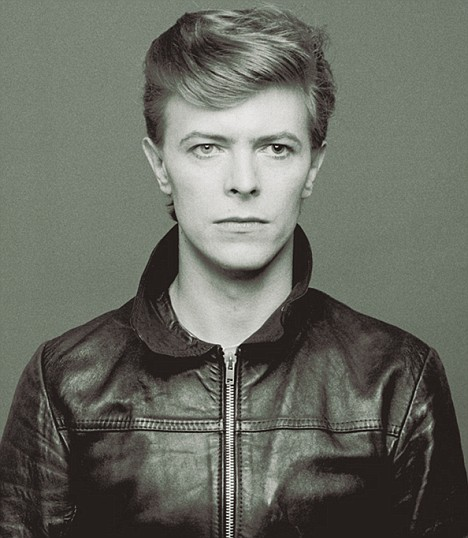
\includegraphics[width=2in,height=2.5in,clip,keepaspectratio]{headshot.jpg}
\end{wrapfigure}

David R. Jones studied art, music and design, including layout and typesetting. After Terry Burns, his half-brother, introduced him to modern jazz, his enthusiasm for players like Charles Mingus and John Coltrane led his mother to give him a plastic alto saxophone in 1961; he was soon receiving lessons from a local musician.

\end{vita}
\end{document}
